  % --------------------------------------------------------------
% This is all preamble stuff that you don't have to worry about.
% Head down to where it says "Start here"
% --------------------------------------------------------------
 
\documentclass[12pt]{article}
 
\usepackage[margin=1in]{geometry} 
\usepackage{amsmath,amsthm,amssymb}
\usepackage[margin=1in]{geometry} 
\usepackage{amsmath,amsthm,amssymb}
\usepackage[english]{babel} 
\usepackage[T1]{fontenc} %escribe lo del teclado
\usepackage[utf8]{inputenc} %Reconoce algunos símbolos
\usepackage{lmodern} %optimiza algunas fuentes
\usepackage{graphicx}
\graphicspath{ {images/} }
\usepackage[urlcolor=blue,colorlinks=true]{hyperref}
\usepackage{makecell}
\usepackage{adjustbox}
\usepackage[justification=centering]{caption}
\usepackage[style=alphabetic]{biblatex}  
\addbibresource{references/papers.bib}  
\setlength{\parindent}{0em} 
\usepackage{listings}
\usepackage{color,soul}
 
\newcommand{\N}{\mathbb{N}}
\newcommand{\Z}{\mathbb{Z}}
 
\newenvironment{theorem}[2][Theorem]{\begin{trivlist}
\item[\hskip \labelsep {\bfseries #1}\hskip \labelsep {\bfseries #2.}]}{\end{trivlist}}
\newenvironment{lemma}[2][Lemma]{\begin{trivlist}
\item[\hskip \labelsep {\bfseries #1}\hskip \labelsep {\bfseries #2.}]}{\end{trivlist}}
\newenvironment{exercise}[2][Exercise]{\begin{trivlist}
\item[\hskip \labelsep {\bfseries #1}\hskip \labelsep {\bfseries #2.}]}{\end{trivlist}}
\newenvironment{problem}[2][Problem]{\begin{trivlist}
\item[\hskip \labelsep {\bfseries #1}\hskip \labelsep {\bfseries #2.}]}{\end{trivlist}}
\newenvironment{question}[2][Question]{\begin{trivlist}
\item[\hskip \labelsep {\bfseries #1}\hskip \labelsep {\bfseries #2.}]}{\end{trivlist}}
\newenvironment{corollary}[2][Corollary]{\begin{trivlist}
\item[\hskip \labelsep {\bfseries #1}\hskip \labelsep {\bfseries #2.}]}{\end{trivlist}}

\newenvironment{solution}{\begin{proof}[Solution]}{\end{proof}}
 
\begin{document}
 
% --------------------------------------------------------------
%                         Start here
% --------------------------------------------------------------
 
\title{Green Orbital Propulsion System for a Small Satellite}
\author{Christian Molli\`ere\\Luca Irtingkauf\\Christian Strohl}
\maketitle
\newpage

% B1
\section{Reference Case Definition}
\label{chap:reference_case}
Most the orbital propulsion systems used for AOCS tasks do not need to provide a very high amount of $\Delta v$ to the satellite bus. Therefore, lightweight and simple blow-down feed systems (see Figure \ref{fig:blowdown_system}) are usually implemented to supply the propellant to the engines. Usually an injector is used to evenly distribute the fuel within the combustion chamber leading to a pressure loss of $\Delta p_{\text{injector}}$ along the fuel line.\\

\begin{figure}[!h]
	\centering
	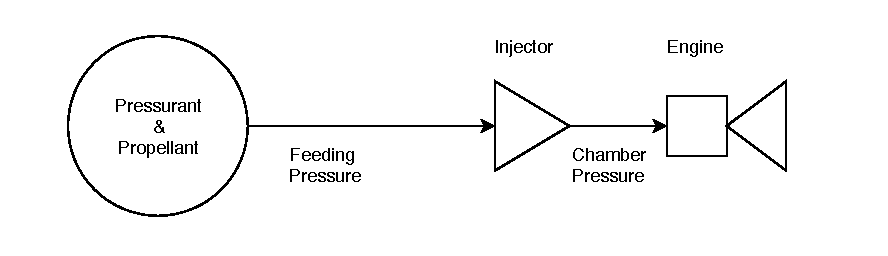
\includegraphics[width=\linewidth]{figures/blowdown_sketch}
	\caption{Simplified view of a pressure blow down system used to transport propellant to the engine. The pressurant and the propellant are separated by a diaphragm.}
	\label{fig:blowdown_system}
\end{figure}

We will assume the following injection pressure loss, since neither the chamber pressure $p_c$ nor the pressure loss at the injector $\Delta p_{\text{injector}}$ are commonly cited in propulsion system specifications.
\begin{equation}
	\Delta p_{\text{injector}} \approx \frac{1}{2}p_c 
	\label{eq:injector_loss_assumption}
\end{equation}

This will lead to an estimated chamber pressure using Equation (\ref{eq:injector_loss_assumption}) as shown in the following.
\begin{gather}
	p_{\text{feed}} = p_c + \Delta p_{\text{injector}} \\
	\rightarrow \quad p_c \approx \frac{2}{3} p_{\text{feed}}
	\label{eq:chamber_pressure_estimation}
\end{gather}

During our internet research the propulsion systems in Table \ref{tab:reference} were found. All systems use monopropellants and are used for AOCS tasks of the spacecraft. In the following we will use the \textbf{XMM Thruster} as a reference case using a feeding pressure of $p_{\text{feed}}=5.5\text{bar}-24\text{bar}$ and a nozzle expansion ratio of $\epsilon=60$.\\

\begin{table}[h!]
	\centering
	\begin{tabular}{|c|c|c|c|}
		\hline
		Case & \makecell{Chamber\\ Pressure {[}bar{]}} & Expansion Ratio & \makecell{Initial Propellant\\ Temperature {[}K{]}} \\ \hline
		XMM Thruster                      &        3.67-16         &  60   &              293.15                      \\ \hline
	\end{tabular}
	\caption{Parameters needed for NASA CEA calculations based on the reference case of the XMM Thruster system.}
	\label{tab:selected_reference_case}
\end{table}

Using Equation (\ref{eq:chamber_pressure_estimation}) we can translate the feeding pressure of the XMM Thruster system to a chamber pressure of $p_{c}=3.67\text{bar}-16\text{bar}$. Furthermore, an initial propellant temperature of $20^\circ\text{C}$ was assumed for all calculations. The reference case is summarized in Table \ref{tab:selected_reference_case}.
 
% B2
\section{Propellants Comparision}
Using the parameters of the reference case in Table \ref{tab:selected_reference_case}, the following green propellants in Table \ref{tab:comparison} were investigated using NASA CEA. The reaction products were set to frozen from the nozzle on outwards, to prevent further reaction in the nozzle as demanded in the task description.

\begin{table}[!h]
	\centering
	\begin{tabular}{|c|c|c|}
		\hline
		Propellant & Vacuum Specific Impulse {[}s{]} & Combustion Temperature {[}K{]} \\ \hline
		LMP-103S   & 253.2 & 1864-1865  \\ \hline
		AF-M315E   & 261  & 2102-2105  \\ \hline
		H2O2, 98\% & 188   & 1225    \\ \hline     
	\end{tabular}\\
	\caption{Comparison of green propellants to the reference case. Each calculation is done using the minimum and maximum feeding pressure of the reference case. If only one result is displayed no difference was calculated between max. and min. chamber pressure.}
	\label{tab:comparison}
\end{table}

% B3
\section{Propellant Optimization}
\label{chap:task_b3}
To optimize the propellant composition of Methanol, ADN and Water a rocketCEA script was written in Python. It performs a search on a composition grid, with a step size of $1\%$ weight fraction. It iterates through all possible composition permutations. The input parameters were taken from the reference case in Table \ref{tab:selected_reference_case} using only the maximum chamber pressure. The results are discussed in the following.

\paragraph{All results}
The top figure in Figure \ref{fig:fuel_optimization_all_results} shows the result of the optimization with a maximum specific impulse in vacuum of $I_{sp}=301.43s$ using $17\%$ of Methanol, $83\%$ ADN and $0\%$ Water.

\paragraph{Final result}
The task demanded a combustion temperature below 1000$^\circ$C (1273.15K). Hence, all results with a higher combustion temperature were removed from the lower figure of Figure \ref{fig:fuel_optimization_all_results}. This lead to the final result with a maximum specific impulse in vacuum of $I_{sp}=236.50s$ using $39\%$ of Methanol, $59\%$ ADN and $2\%$ Water.\\

Additionally, we need to consider that solid ADN will need to be dissolved in the other two components of the propellant. At a temperature of $20^\circ C$, which is coherent with our initial propellant temperature, $356\text{g}$ ADN can be dissolved in $100\text{g}$ of Water and $86\text{g}$ ADN can be dissolved in $100\text{g}$ Methanol \cite{Larsson2011}.\\

\hl{Literaturwerte: 357g und 86,9g!}

According to this data, the used $39\%$ Methanol can dissolve $33.54\%$ of ADN. The remaining $25.46\%$ of ADN would need to be dissolved by the propellants $2\%$ of Water, which can only dissolve $7.12\%$ of ADN at a temperature of 20$^\circ$C. Therefore, the found propellant composition would contain $18.34\%$ of solid ADN rendering it unusable in real engines, because the solids are likely to cause problems in the feeding systems and would lead to inhomogenous mixtures in the combustion chamber.\\

Optimizing the propellant composition to comply with the mentioned solubility constraint is beyond the scope of this task and shall only be mentioned here.

% B4
\section{Thruster Preliminary Design}
The new propulsion system should provide the same amount of thrust as the reference case being 20N. With thrust $F$ being defined as
\begin{equation}
	F = I_{sp} \cdot \dot{m}_{\text{prop}} \cdot g \overset{!}{=} 20\text{N}.
	\label{eq:thrust}
\end{equation}
Therefore, the required mass flow rate $\dot{m}_{\text{prop}}$ is calculated using the earth's gravitational acceleration of $g=9.81\frac{m}{s^2}$ and the in task B3 determined specific impulse of $I_{sp}=236.5s$.
\begin{equation*}
	\dot{m}_{\text{prop}} = 0.00862 \frac{\text{kg}}{\text{s}} = 8.62 \frac{\text{g}}{\text{s}}
\end{equation*}
To reach the same amount of total impulse $I_{\text{total}}=517000\text{Ns}$ (see Table \ref{tab:reference}) the propellant mass $m_{\text{prop}}$ can be calculated to be
\begin{equation*}
	m_{\text{prop}} = \frac{I_{\text{Total}}}{F} \cdot \dot{m}_{\text{prop}} =  211.97\text{kg}.
\end{equation*}
Using NASA CEA the complete output is computed for the propellant composition found in Section \ref{chap:task_b3}. It can be found on Page \pageref{chap:cea_output} to obtain the characteristic exhaust speed $c^*=4240.4\frac{\text{ft}}{\text{s}}=1292.5\frac{\text{m}}{\text{s}}$. From here we are able to calculate appropriate throat area $A_t$ to
\begin{equation}
	A_t = \frac{c^* \cdot \dot{m}_{\text{prop}}}{p_c} = 6.96 \cdot 10^{-6} \text{m}^2.
	\label{eq:throat_ares}
\end{equation}
Using the expansion ratio $\epsilon=60$ this leads to a nozzle exit area $A_e$ of
\begin{equation*}
A_e = \epsilon * A_t = 4.18 \cdot 10^{-4} \text{m}^2.
\end{equation*}

% B5
\section{Detailed Design Blow-Down Feed System}
Combining Equation \ref{eq:thrust} and Equation \ref{eq:throat_ares} the produced thrust of the optimized propellant can be studied for varying chamber pressures $p_c$ as seen in Equation \ref{eq:thrust_vs_pc}.
\begin{equation}
	F = I_{sp} \cdot g \cdot \frac{A_t\cdot p_c}{c^*}
	\label{eq:thrust_vs_pc}
\end{equation}
We want the engine to retain at least a quarter of its thrust, being $F_{\text{EOL}}=5\text{N}$, at the end of its life. According to our calculations (see Figure \ref{fig:thrust_vs_pc}) the engine will linearly loss thrust with decreasing chamber pressures. Therefore, an end of life chamber pressure of $p_{c,\text{EOL}}=4\text{bar}$ is defined. Furthermore, the chamber pressure at mission launch can defined to be the same as in the reference case $p_{c,\text{BOL}}=16\text{bar}$.\\

\begin{figure}[h]
	\centering
	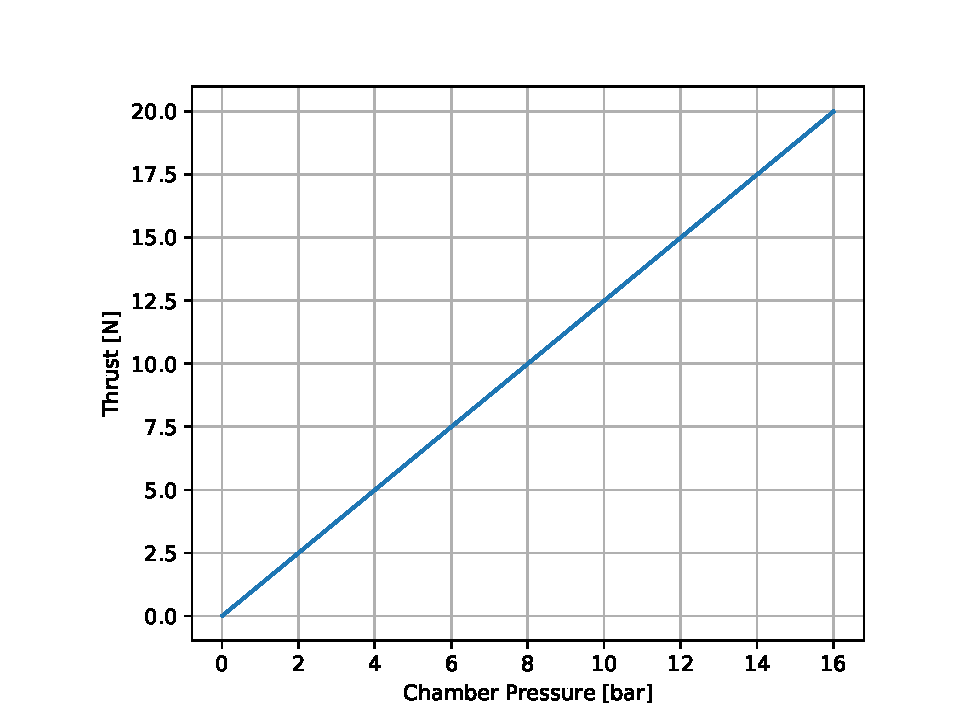
\includegraphics[width=0.8\linewidth]{figures/thrust_vs_pc.pdf}
	\caption{The optimized propellants thrust in vacuum at different chamber pressures.}
	\label{fig:thrust_vs_pc}
\end{figure}

Since it is the simplest and cheapest design, a blow-down feed system is used to feed the propellant to the engine. Assuming the same pressure loss at the fuel injector $\Delta p_{\text{injector}}= \frac{p_c}{2}$ as in Section \ref{chap:reference_case} leads to feeding pressures of $p_{feed,\text{BOL}}=24\text{bar}$ and $p_{feed,\text{EOL}}=6\text{bar}$.\\

To achieve an even greener propulsion system, we decided to use Nitrogen instead of Helium to pressurize the propellant. Considering the global shortage of Helium this will ensure a sustainable propulsion system for years to come. The final feeding system architecture can be seen in Figure \ref{fig:blowdown_design}.\\

\begin{figure}[h]
	\centering
	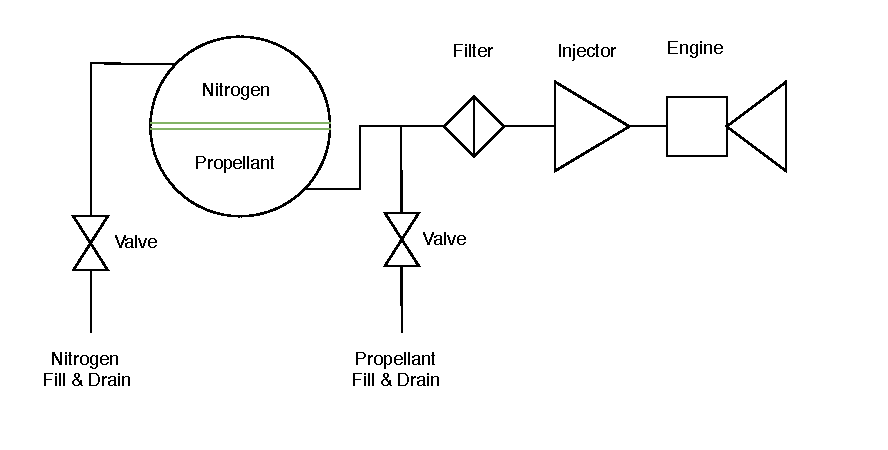
\includegraphics[width=\linewidth]{figures/blowdown_design.pdf}
	\caption{Final design of the blow down feeding system for the green orbital propulsion system.}
	\label{fig:blowdown_design}
\end{figure}

In order to Calculate the amount of needed pressurant, we will need to estimate the density of the used propellant. According to this lectures exercise 3 from the 27.06.2019, the green propellant LMP-103S has a density of $\rho_{\text{LMP}}=1250 \frac{kg}{m^3}$. Its composition is quite similar to the here optimized propellant. Thus, the propellants density is estimated to be
\begin{equation*}
	\rho_{\text{prop}} \approx \rho_{\text{LMP}}=1250 \frac{kg}{m^3}.
\end{equation*}
This leads to a propellant volume of 
\begin{equation*}
V_{\text{prop}} = m_{\text{prop}} / \rho_{\text{prop}} = 0.1696 \text{m}^3.
\end{equation*}
Now the needed amount of pressurant can be calculated using the ideal gas equation and taking into account that the tank volume is constant. Moreover, we assume that the propellant is only released in short bursts which will keep the propellant temperature constant at the initial temperature of $T_0=20^\circ\text{C}$.
\begin{equation}
V_{\text{tank}} = \frac{m_{N2} R_{N2} T_0}{p_{feed,\text{BOL}}} + V_{\text{prop}} = \frac{m_{N2} R_{N2} T_0}{p_{feed,\text{EOL}}}
\label{eq:tank_mass_equilibrium}
\end{equation}
Using the molecular mass of Nitrogen $M_{N2}=28.01340\frac{\text{g}}{\text{mol}}$, its specific ideal gas constant can be determined to be $R_{N2}=296.78 \frac{\text{J}}{\text{kg K}}$.
Solving Equation \ref{eq:tank_mass_equilibrium} results in a pressurant mass of
\begin{equation*}
	m_{N2} = 1.56kg.
\end{equation*}
In comparison, using Helium with a specific ideal gas constant of $R_{He}=2078.5 \frac{\text{J}}{\text{kg K}}$, we would only need $m_{He}=0.223kg$ of pressurant.\\

Then, we can calculate the dimensions of the combined pressurant and propellant tank using Equation \ref{eq:chamber_pressure_estimation} to be
\begin{equation*}
	V_{\text{tank}} = 0.226\text{m}^3.
\end{equation*}
Which leads to a tank radius $r$, assuming the use of a spherical tank, of
\begin{equation*}
	r = \sqrt[3]{\frac{3}{4\pi} V_{\text{tank}}} = 0.377m
\end{equation*}
Using Titanium with a maximum allowed operating stress of $S_{Ti}=6894.75\text{bar}$ we can estimate the tank thickness $t$ with a safety factor of 2 to
\begin{equation*}
	t = \frac{p_{feed,\text{BOL}}\cdot r}{4 \cdot S_{Ti}} = 0.329\text{mm}
\end{equation*}
Finally the empty tank mass is calculated using a Titanium density of $\rho=4430\frac{\text{kg}}{\text{m}^3}$
\begin{equation*}
	m_{\text{tank}} = \rho_{Ti} \cdot \frac{4}{3} \pi ((r+t)^3 - r^3) = 2.605kg
\end{equation*}
The complete system mass will further need to include several engines, valves, fuel lines and filters. Estimating a mass of the residual parts of $m_{\text{res}} \approx 15\text{kg}$, the complete system mass adds up to 
\begin{equation*}
m_{\text{system}} = m_{\text{tank}} + m_{\text{prop}} + m_{\text{N2}} + m_{\text{res}} = 231.135\text{kg}.
\end{equation*}
Since the system has a rather high amount of propellant it should be able to propell the spacecraft for longer mission durations in orbit.

% Optimzation results
\newpage
\begin{figure}[!h]
	\centering
	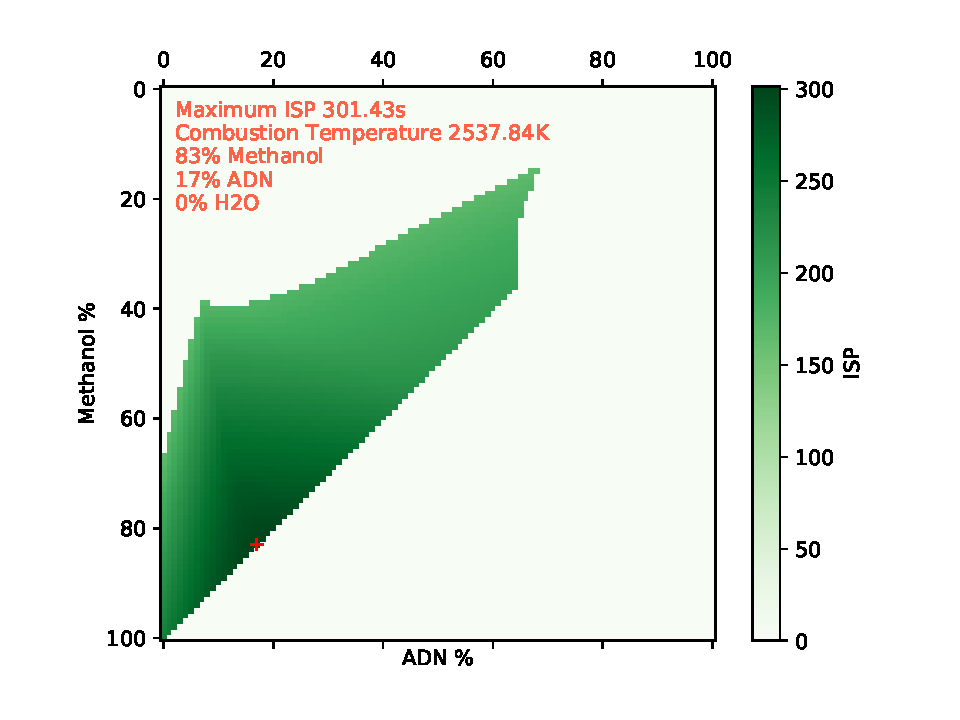
\includegraphics[width=0.8\linewidth]{figures/b3_1.pdf}
	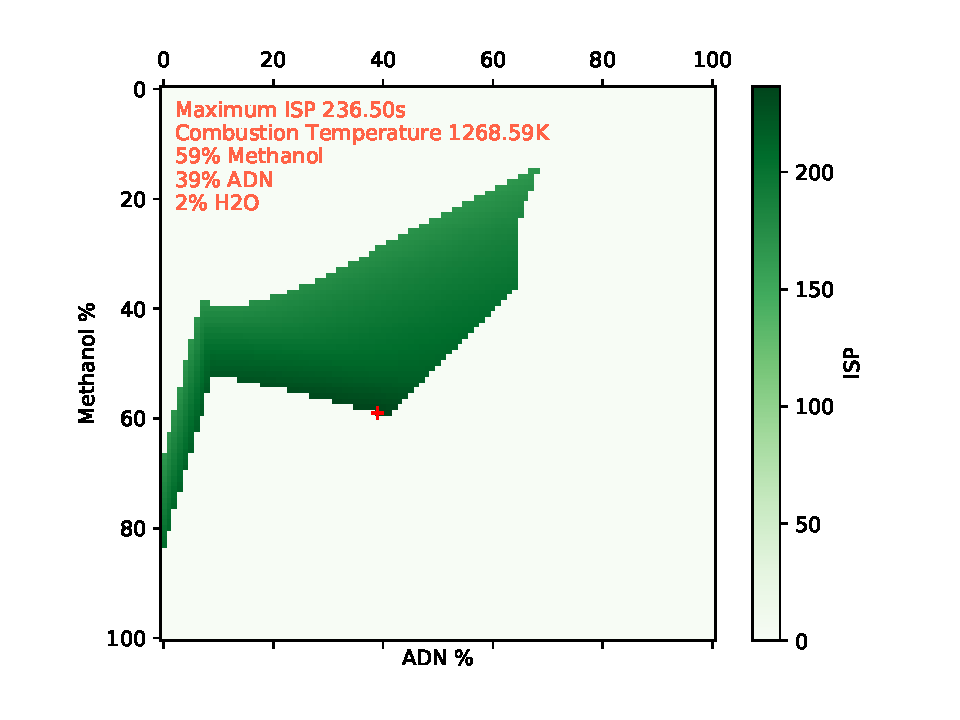
\includegraphics[width=0.8\linewidth]{figures/b3_2.pdf}
	\caption{Figure showing the fuel optimization using Nasa CEA to compute the highest possible ISP (top). The best results are highlighted with a red cross. The second figure shows the best result after all reactions with a combustion temperature above 1000$^\circ$C (1273.15K) are removed (bottom).}
	\label{fig:fuel_optimization_all_results}
\end{figure}

% Overview
\newpage
\begin{adjustbox}{angle=90, center,caption={Overview of small propulsion systems using monopropellants.}}%,float=table}
	\begin{tabular}{|c|c|c|c|c|c|c|}
		\hline
		Name & Propellants & \makecell{Number of\\Thrusters} & \makecell{Thruster\\Class {[}N{]}} & \makecell{Total\\Impulse [Ns]} & Other & References\\ \hline
		
		\makecell{XMM\\Thruster} & N2H4 & 8 & 20 & \makecell{$>517000$}  & \makecell{$I_{sp}=222-230s$,\\$p_{\text{feed}}=5.5-24\text{bar}$,\\$\epsilon=60$} & \makecell{ \cite{EsaXMM} \cite{ariane20N}} \\ \hline
		
		\makecell{TanDEM-X\\Thruster} & \makecell{N2H4} & 4 & 1 & \makecell{$>135000$}& \makecell{$I_{sp}=200-223s$,\\$p_{\text{feed}}=5.5-22\text{bar}$,\\$\epsilon=80$\\} & \makecell{\cite{tandemX} \cite{ariane1N}}\\ \hline
		
		\makecell{Prisma\\Thruster}& LMP-103S & 2 & 1 & \makecell{$\approx 108773$} & \makecell{$I_{sp}=204-231s$,\\$p_{\text{feed}}=4.5-22\text{bar}$,\\$\epsilon=100$} & \cite{hpgpThruster} \\ \hline
	\end{tabular}
	\label{tab:reference}
\end{adjustbox}

% Appendix
\newpage
\section{NASA CEA Output for Optimized Propellant}
\label{chap:cea_output}
\lstinputlisting{results/b4.out}

% References
\newpage
\printbibliography 
 
\end{document}
